\documentclass[12pt]{article}
\usepackage[a4paper, margin=1in]{geometry}
\usepackage{times}
\usepackage{graphicx}
\usepackage{tikz}
\usetikzlibrary{shapes.geometric, arrows.meta, positioning, calc}
\usepackage{cite}
\usepackage{setspace}
\usepackage{titlesec}
\usepackage{hyperref}

\onehalfspacing

\titleformat{\section}{\large\bfseries\scshape}{\thesection.}{1em}{}
\titleformat{\subsection}{\normalsize\bfseries}{\thesubsection.}{1em}{}

\begin{document}

\begin{center}
    {\LARGE \textbf{DefectLens: Efficient ViT-Based Anomaly Detection with Multi-Criteria Token Fusion (MCTF)} \par}
    \vspace{0.5cm}
    {\large \textbf{Tanish Babu} \par}
    {\large Roll No: 2023bcs0067 \par}
    {\large Computer Vision Course Project \par}
    {\large Weekly Project Write-Up \par}
    \vspace{0.5cm}
\end{center}

\begin{abstract}
\noindent This document presents the foundational context and system architecture for the DefectLens project. It explores the computational bottlenecks associated with deploying Vision Transformers (ViTs) for high-resolution industrial anomaly detection. Furthermore, it outlines the rationale for utilizing a Multi-Criteria Token Fusion (MCTF) module to achieve real-time inference on edge devices, along with the specific project goals designed to balance high detection accuracy with low latency in automated inspection pipelines.
\end{abstract}

\vspace{0.5cm}

\section{Problem Statement}
In the realm of manufacturing quality control, reliable visual inspection is essential. Conventional supervised learning methods fall short because they demand massive amounts of labeled data for every possible defect. Since manufacturing defects are rare and unpredictable, collecting such data is highly impractical. As a result, unsupervised anomaly detection---which involves modeling the distribution of flawless products---has become the preferred approach.

Vision Transformers (ViTs) have recently demonstrated exceptional capabilities in anomaly detection by capturing global image contexts alongside detailed patch-level features. However, they suffer from severe computational costs that scale quadratically with sequence length. In industrial environments, where fast processing (low latency) and high-resolution inputs are non-negotiable, the rigid and redundant token processing mechanism of standard ViTs creates a significant bottleneck.

The primary problem this project seeks to resolve is: \textit{How can we dramatically decrease the computational demands of ViTs for anomaly detection while retaining the high-resolution, localized visual information needed to accurately detect minute defects?}

\section{Motivation and Intended Application}
The inability to detect minor defects can result in severe consequences, including product recalls, safety risks, and financial losses, especially in high-precision sectors like semiconductor and aerospace manufacturing. On the other hand, if an inspection system is too slow, it becomes a production bottleneck that severely limits output. Balancing this latency-accuracy trade-off is a critical challenge in advancing Industry 4.0 and smart manufacturing.

Our motivation is driven by the strict operational requirements of modern assembly lines, which demand both high accuracy and minimal processing time. While traditional CNNs struggle with modeling complex global textures, unoptimized ViTs are simply too slow for deployment on real-time edge hardware.

\textbf{Intended Application:} This solution is tailored for Automated Optical Inspection (AOI) systems integrated directly into factory production lines. Utilizing this optimized anomaly detection model, manufacturers can automatically spot structural flaws, surface blemishes, and assembly mistakes (similar to categories in the MVTec AD dataset) in real-time as items move down a high-speed conveyor.

\section{Project Objectives}
The main goal of the DefectLens project is to develop an efficient, high-throughput industrial anomaly detection system that leverages the robust feature extraction of Vision Transformers while mitigating their computational overhead. Specifically, the objectives are:

\begin{itemize}
    \item \textbf{Baseline Implementation:} Construct a Vision Transformer backbone paired with a PatchCore-style Memory Bank to serve as a strong baseline for unsupervised anomaly detection.
    \item \textbf{Token Fusion Integration:} Incorporate a Multi-Criteria Token Fusion (MCTF) module that intelligently merges redundant background tokens across the ViT layers, inspired by the methodology of Lee et al. \cite{lee2023multi}.
    \item \textbf{Feature Preservation:} Apply specific criteria---such as token similarity, one-step-ahead attention informativeness, and size penalties---to guarantee that small but vital defect features are not accidentally fused into the background.
    \item \textbf{Latency Reduction:} Significantly lower the Floating Point Operations (FLOPs) and overall inference time by cutting down the number of processed tokens, enabling high-speed edge deployment.
    \item \textbf{Full System Deployment:} Wrap the underlying model within a complete application stack, featuring a FastAPI backend and a React frontend, to simulate a realistic quality control interface for factory operators.
\end{itemize}

\section{System Architecture Diagram}
To execute the token reduction strategy without compromising accuracy, the MCTF module is placed between the layers of the Vision Transformer. Figure \ref{fig:architecture} illustrates the high-level workflow from the initial image capture down to the final anomaly heatmap.

\begin{figure}[htpb]
    \centering
    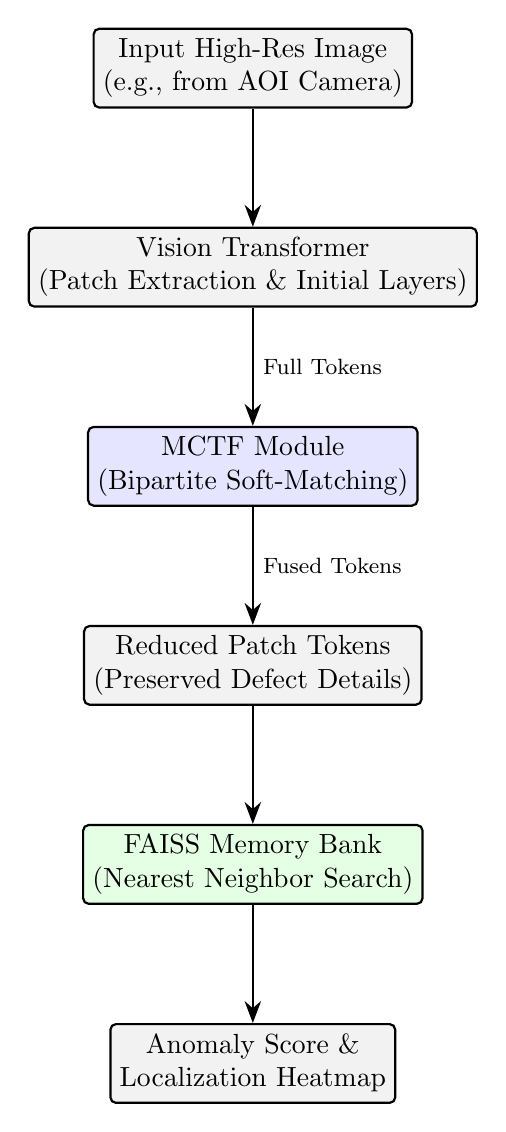
\begin{tikzpicture}[
        node distance=1.5cm and 1cm,
        box/.style={rectangle, draw=black, thick, minimum width=3.5cm, minimum height=1cm, align=center, fill=gray!10, rounded corners=2pt},
        arrow/.style={-{Stealth[scale=1.2]}, thick}
    ]
        % Nodes
        \node[box] (input) {Input High-Res Image \\ (e.g., from AOI Camera)};
        \node[box, below=of input] (vit) {Vision Transformer \\ (Patch Extraction \& Initial Layers)};
        \node[box, below=of vit, fill=blue!10] (mctf) {MCTF Module \\ (Bipartite Soft-Matching)};
        \node[box, below=of mctf] (fused) {Reduced Patch Tokens \\ (Preserved Defect Details)};
        \node[box, below=of fused, fill=green!10] (memory) {FAISS Memory Bank \\ (Nearest Neighbor Search)};
        \node[box, below=of memory] (output) {Anomaly Score \& \\ Localization Heatmap};

        % Arrows
        \draw[arrow] (input) -- (vit);
        \draw[arrow] (vit) -- node[right, font=\footnotesize] {Full Tokens} (mctf);
        \draw[arrow] (mctf) -- node[right, font=\footnotesize] {Fused Tokens} (fused);
        \draw[arrow] (fused) -- (memory);
        \draw[arrow] (memory) -- (output);
    \end{tikzpicture}
    \caption{High-Level Architecture of DefectLens integrating MCTF.}
    \label{fig:architecture}
\end{figure}

\section{Core Ideas and References}
This project is deeply rooted in recent advancements in token reduction for Vision Transformers. The token fusion algorithm heavily relies on the innovative concepts presented by Lee et al. \cite{lee2023multi}. Their introduction of ``one-step-ahead attention'' provides a crucial mechanism to evaluate token informativeness, allowing the model to shield highly relevant tokens from being fused. This ensures that the subtle visual indicators of manufacturing defects are maintained throughout the network.

\begin{thebibliography}{9}
\bibitem{lee2023multi}
Sanghyeok Lee, Joonmyung Choi, and Hyunwoo J. Kim,
\textit{``Multi-criteria Token Fusion with One-step-ahead Attention for Efficient Vision Transformers,''}
Department of Computer Science and Engineering, Korea University.
Emails: \{cat0626, pizard, hyunwoojkim\}@korea.ac.kr.
\end{thebibliography}

\end{document}
